\subsection{Case study \#2: Flowlet size distributions}
\label{s:eval:mininet-flowlet}
\label{sec:eval:mininet-flowlet}

We demonstrate another use case for Marple in practice: computing the flowlet
size distribution as a function of the flowlet
\emph{threshold}, the time gap above which subsequent packets are considered to
be in different flowlets.
This analysis has many
practical uses, \eg for configuring flowlet-based load balancing
strategies~\cite{conga, letflow}.
In particular, the performance of LetFlow~\cite{letflow} depends heavily
on the distribution of flowlet sizes. 

Our setup uses Mininet with a single-switch connecting five hosts: a single
client and four servers. Flow sizes are drawn from an empirical distribution
computed from a trace of a real data center~\cite{empirical-flow-data}.  The
switch runs the ``flowlet size histogram'' query from
\Fig{example-perf-queries} for six values of {\ct delta}, the flowlet
threshold.

\Fig{flowletcdf} shows the CDF of flowlet sizes for various values of {\ct
delta}. Note that the actual values of {\ct delta} are a consequence of the
bandwidth allowed by the Mininet setup; a data center deployment would likely
use much lower {\ct delta} values.

\begin{figure}[!t]
\centering
\vspace{-0.2in}
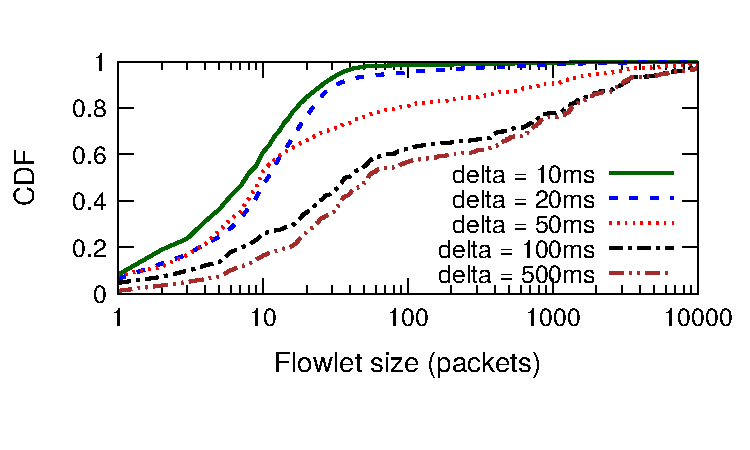
\includegraphics[width=0.8\columnwidth]{pq_flowlet-cdf.pdf}
\vspace{-0.3in}
\caption{CDF of flowlet sizes for different flowlet thresholds.}
\vspace{-0.15in}
\label{fig:flowletcdf}
\end{figure}
